\documentclass{beamer}\usepackage[]{graphicx}\usepackage[]{color}
%% maxwidth is the original width if it is less than linewidth
%% otherwise use linewidth (to make sure the graphics do not exceed the margin)
\makeatletter
\def\maxwidth{ %
  \ifdim\Gin@nat@width>\linewidth
    \linewidth
  \else
    \Gin@nat@width
  \fi
}
\makeatother

\definecolor{fgcolor}{rgb}{0, 0, 0}
\newcommand{\hlnum}[1]{\textcolor[rgb]{0.533,0,0.133}{#1}}%
\newcommand{\hlstr}[1]{\textcolor[rgb]{0.667,0.267,0}{#1}}%
\newcommand{\hlcom}[1]{\textcolor[rgb]{1,0.533,0}{#1}}%
\newcommand{\hlopt}[1]{\textcolor[rgb]{0,0,0}{\textbf{#1}}}%
\newcommand{\hlstd}[1]{\textcolor[rgb]{0,0,0}{#1}}%
\newcommand{\hlkwa}[1]{\textcolor[rgb]{0.4,0.067,0.067}{\textbf{#1}}}%
\newcommand{\hlkwb}[1]{\textcolor[rgb]{0,0,0.4}{\textbf{#1}}}%
\newcommand{\hlkwc}[1]{\textcolor[rgb]{0,0,0.4}{#1}}%
\newcommand{\hlkwd}[1]{\textcolor[rgb]{0,0.267,0.4}{#1}}%
\let\hlipl\hlkwb

\usepackage{framed}
\makeatletter
\newenvironment{kframe}{%
 \def\at@end@of@kframe{}%
 \ifinner\ifhmode%
  \def\at@end@of@kframe{\end{minipage}}%
  \begin{minipage}{\columnwidth}%
 \fi\fi%
 \def\FrameCommand##1{\hskip\@totalleftmargin \hskip-\fboxsep
 \colorbox{shadecolor}{##1}\hskip-\fboxsep
     % There is no \\@totalrightmargin, so:
     \hskip-\linewidth \hskip-\@totalleftmargin \hskip\columnwidth}%
 \MakeFramed {\advance\hsize-\width
   \@totalleftmargin\z@ \linewidth\hsize
   \@setminipage}}%
 {\par\unskip\endMakeFramed%
 \at@end@of@kframe}
\makeatother

\definecolor{shadecolor}{rgb}{.97, .97, .97}
\definecolor{messagecolor}{rgb}{0, 0, 0}
\definecolor{warningcolor}{rgb}{1, 0, 1}
\definecolor{errorcolor}{rgb}{1, 0, 0}
\newenvironment{knitrout}{}{} % an empty environment to be redefined in TeX

\usepackage{alltt}
\newenvironment{changemargin}[2]{%
\begin{list}{}{%
\setlength{\topsep}{0pt}%
\setlength{\leftmargin}{#1}%
\setlength{\rightmargin}{#2}%
\setlength{\listparindent}{\parindent}%
\setlength{\itemindent}{\parindent}%
\setlength{\parsep}{\parskip}%
}%
\item[]}{\end{list}}
\usepackage{graphicx}
\usepackage{amsmath}
\usepackage{url}
\usetheme{Madrid}
\usecolortheme{beaver}
\setbeamertemplate{navigation symbols}{}
\titlegraphic{
\includegraphics[width=5cm]{..//..//S-DS-VC-RGB.png}}
%\logo{
\includegraphics[width=0.1\textwidth,keepaspectratio]{..//..//UOACrest.png}}
\author[SCC]{Statistical Consulting Centre}%\\
\institute[\href{mailto:consulting@stat.auckland.ac.nz}
  {consulting@stat.auckland.ac.nz}]{\href{mailto:consulting@stat.auckland.ac.nz}
  {consulting@stat.auckland.ac.nz}\\
%Statistical Consulting Centre\\
The Department of Statistics\\
The University of Auckland}
\title[Session 6 -- Advanced Graphics]{NZSSN Courses: Introduction
to \texttt{R}}
\subtitle{Session 6 -- Advanced Graphics}
\date{15 November, 2016}
\IfFileExists{upquote.sty}{\usepackage{upquote}}{}
\begin{document}
%\SweaveOpts{concordance=TRUE}
\maketitle
 
\begin{frame}[fragile]
  \frametitle{Plot means in context}

\begin{knitrout}
\definecolor{shadecolor}{rgb}{0.965, 0.965, 0.965}\color{fgcolor}\begin{kframe}
\begin{alltt}
\hlkwd{with}\hlstd{(issp.df,} \hlkwd{tapply}\hlstd{(total.lik, age.group,}
                     \hlstd{mean,} \hlkwc{na.rm} \hlstd{=} \hlnum{TRUE}\hlstd{))}
\end{alltt}
\begin{verbatim}
Under 35 36 to 60  Over 61 
13.38871 12.45516 10.78836 
\end{verbatim}
\end{kframe}
\end{knitrout}
\begin{itemize}
\item Means are all but meaningless unless they are presented in context.
\item Always present with standard deviations (SDs) or standard errors of means (SEs) or confidence intervals.
\item Plot means with 95\% confidence intervals ($\pm$ 1.96 $\times$ SE).
\begin{itemize}
\item $\pm$ 1 $\times$ SE yields (approx.) a 68\% confidence interval. Equivalent to using a 16\% level of significance!!!!
\item $\pm$ 1 $\times$ SD tells us \textbf{ABSOLUTELY NOTHING} about whether two means are statistically different from one another.
\end{itemize}
\end{itemize}
\end{frame} 

\begin{frame}[fragile]
  \frametitle{Calculating 95\% CIs}
\begin{itemize}
\item 95\% CI $=$ Mean $\pm$ 1.96 $\times$ SE
\item Standard Errors $= \frac{\text{Standard Deviation}}{\sqrt{\text{Sample Size}}}$
\end{itemize}
\begin{knitrout}
\definecolor{shadecolor}{rgb}{0.965, 0.965, 0.965}\color{fgcolor}\begin{kframe}
\begin{alltt}
\hlstd{my.m} \hlkwb{<-} \hlkwd{with}\hlstd{(issp.df,} \hlkwd{tapply}\hlstd{(total.lik, age.group, mean,}
                             \hlkwc{na.rm} \hlstd{=} \hlnum{TRUE}\hlstd{))}
\hlstd{my.m}
\end{alltt}
\begin{verbatim}
Under 35 36 to 60  Over 61 
13.38871 12.45516 10.78836 
\end{verbatim}
\begin{alltt}
\hlstd{my.sd} \hlkwb{<-} \hlkwd{with}\hlstd{(issp.df,} \hlkwd{tapply}\hlstd{(total.lik, age.group, sd,}
                              \hlkwc{na.rm} \hlstd{=} \hlnum{TRUE}\hlstd{))}
\hlstd{my.sd}
\end{alltt}
\begin{verbatim}
Under 35 36 to 60  Over 61 
2.139623 2.156049 1.964491 
\end{verbatim}
\end{kframe}
\end{knitrout}
\end{frame}


\begin{frame}[fragile]
  \frametitle{Calculating 95\% CIs}
\begin{knitrout}
\definecolor{shadecolor}{rgb}{0.965, 0.965, 0.965}\color{fgcolor}\begin{kframe}
\begin{alltt}
\hlstd{my.n} \hlkwb{<-} \hlkwd{with}\hlstd{(issp.df,} \hlkwd{tapply}\hlstd{(total.lik, age.group,}
            \hlkwa{function}\hlstd{(}\hlkwc{x}\hlstd{)}\hlkwd{length}\hlstd{(}\hlkwd{which}\hlstd{(}\hlopt{!}\hlkwd{is.na}\hlstd{(x)))))}
\hlstd{my.n}
\end{alltt}
\begin{verbatim}
Under 35 36 to 60  Over 61 
     319      446      189 
\end{verbatim}
\begin{alltt}
\hlstd{my.stder} \hlkwb{<-} \hlstd{my.sd}\hlopt{/}\hlkwd{sqrt}\hlstd{(my.n)}
\hlstd{ci.upper} \hlkwb{<-} \hlstd{my.m} \hlopt{+} \hlnum{1.96}\hlopt{*}\hlstd{my.stder}
\hlstd{ci.lower} \hlkwb{<-} \hlstd{my.m} \hlopt{-} \hlnum{1.96}\hlopt{*}\hlstd{my.stder}
\end{alltt}
\end{kframe}
\end{knitrout}
\end{frame}


\begin{frame}[fragile]
  \frametitle{Calculating 95\% CIs}
\begin{knitrout}
\definecolor{shadecolor}{rgb}{0.965, 0.965, 0.965}\color{fgcolor}\begin{kframe}
\begin{alltt}
\hlkwd{cbind}\hlstd{(my.m, ci.lower, ci.upper)}
\end{alltt}
\begin{verbatim}
             my.m ci.lower ci.upper
Under 35 13.38871 13.15391 13.62351
36 to 60 12.45516 12.25506 12.65526
Over 61  10.78836 10.50828 11.06844
\end{verbatim}
\end{kframe}
\end{knitrout}
\end{frame}

\begin{frame}[fragile]
  \frametitle{Plot the means}
\begin{knitrout}
\definecolor{shadecolor}{rgb}{0.965, 0.965, 0.965}\color{fgcolor}\begin{kframe}
\begin{alltt}
\hlkwd{plot}\hlstd{(my.m)}
\end{alltt}
\end{kframe}

{\centering 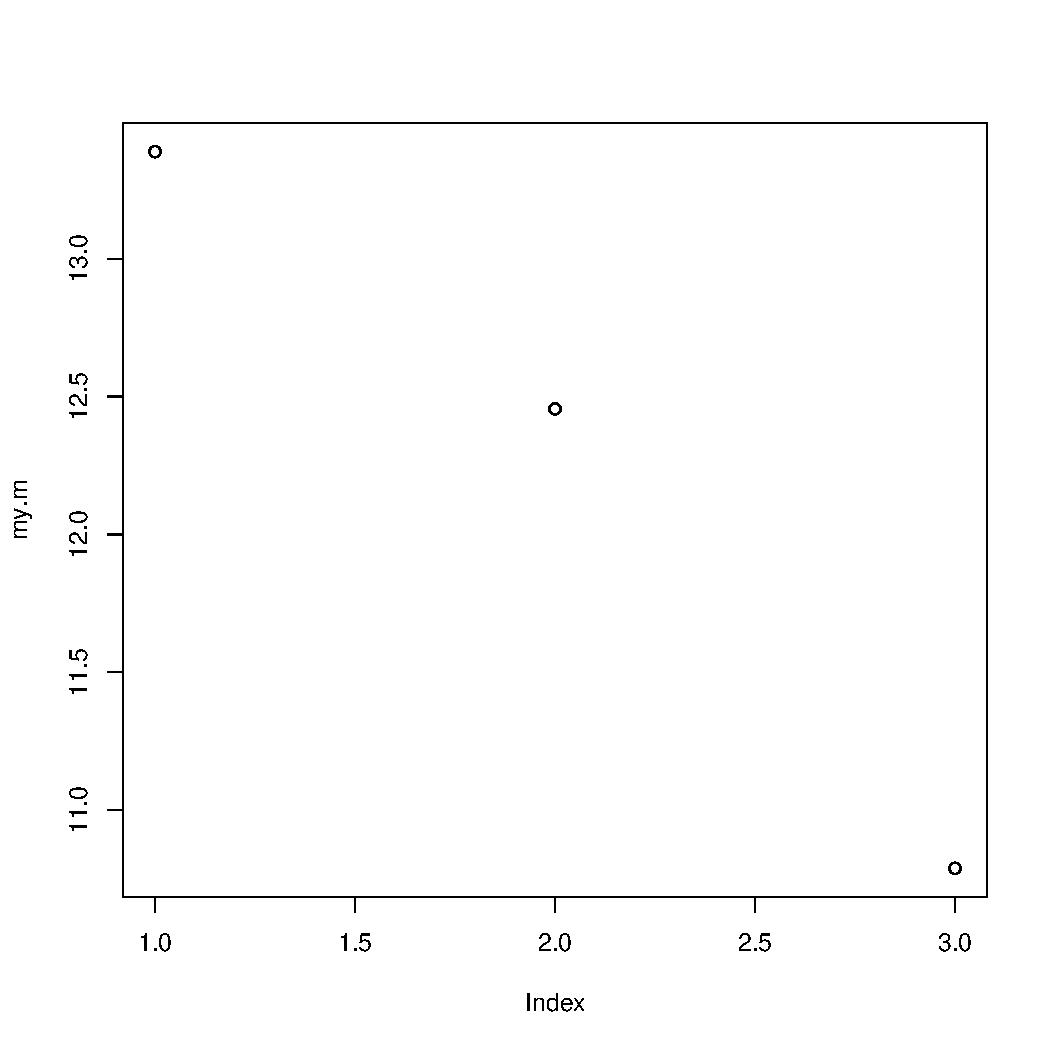
\includegraphics[width=0.6\linewidth]{figure/m1-1} 

}



\end{knitrout}
\end{frame}

\begin{frame}[fragile]
  \frametitle{Make room for the SE bars}
\begin{knitrout}
\definecolor{shadecolor}{rgb}{0.965, 0.965, 0.965}\color{fgcolor}\begin{kframe}
\begin{alltt}
\hlkwd{plot}\hlstd{(my.m,} \hlkwc{ylim} \hlstd{=} \hlkwd{c}\hlstd{(}\hlnum{10}\hlstd{,} \hlnum{14}\hlstd{),} \hlkwc{xlim} \hlstd{=} \hlkwd{c}\hlstd{(}\hlnum{0}\hlstd{,} \hlnum{4}\hlstd{))}
\end{alltt}
\end{kframe}

{\centering 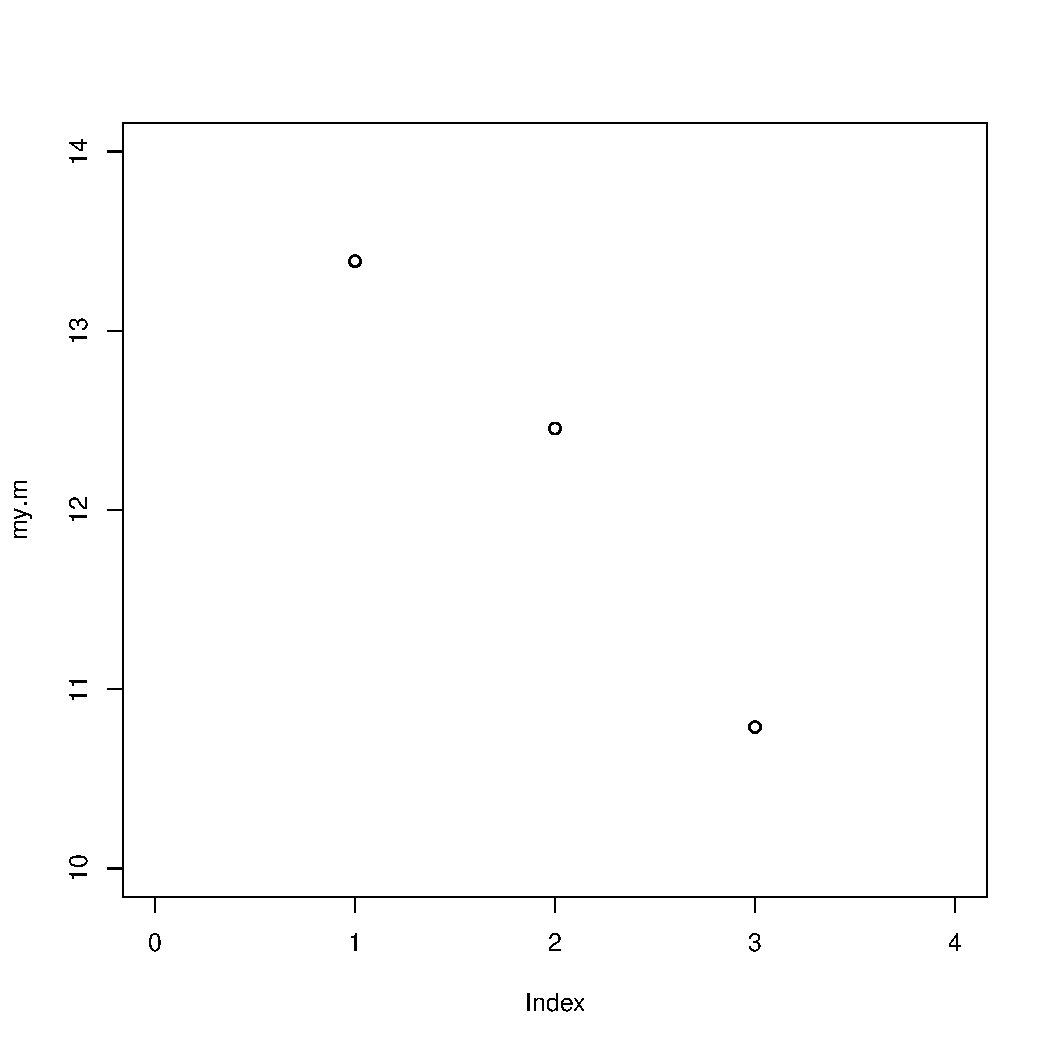
\includegraphics[width=0.6\linewidth]{figure/m2-1} 

}



\end{knitrout}
\end{frame}

\begin{frame}[fragile]
  \frametitle{Adding error bars}
\begin{knitrout}
\definecolor{shadecolor}{rgb}{0.965, 0.965, 0.965}\color{fgcolor}\begin{kframe}
\begin{alltt}
\hlkwd{plot}\hlstd{(my.m,} \hlkwc{ylim} \hlstd{=} \hlkwd{c}\hlstd{(}\hlnum{10}\hlstd{,} \hlnum{14}\hlstd{),} \hlkwc{xlim} \hlstd{=} \hlkwd{c}\hlstd{(}\hlnum{0}\hlstd{,} \hlnum{4}\hlstd{))}
\hlkwd{arrows}\hlstd{(}\hlnum{1}\hlopt{:}\hlnum{3}\hlstd{, ci.lower,} \hlnum{1}\hlopt{:}\hlnum{3}\hlstd{, ci.upper,} \hlkwc{code} \hlstd{=} \hlnum{3}\hlstd{,}
       \hlkwc{angle} \hlstd{=} \hlnum{90}\hlstd{)}
\end{alltt}
\end{kframe}
\end{knitrout}

\begin{figure}[h]
  \vspace{-20pt}
  \centering
  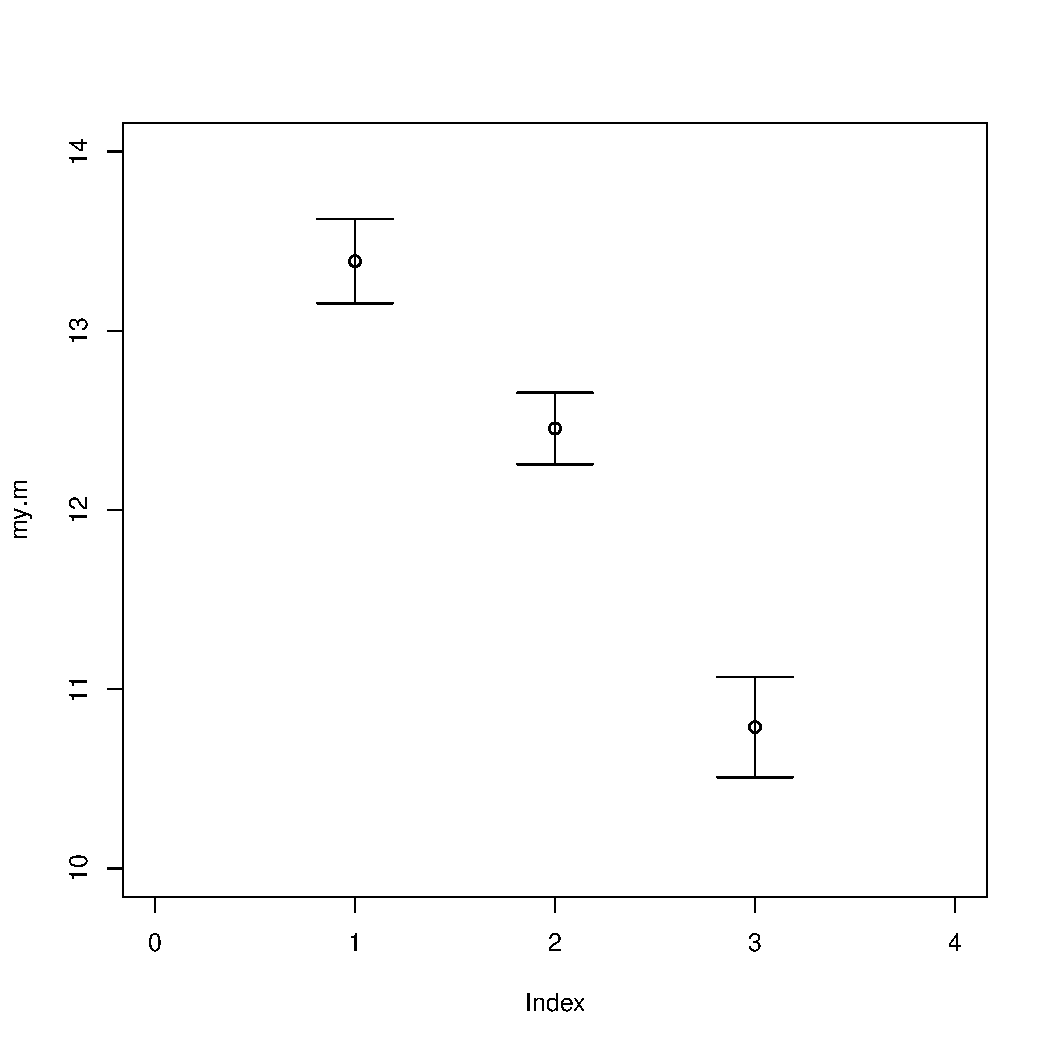
\includegraphics[height = 0.65\textwidth, keepaspectratio]{Figure/m3}
  %\vspace{-20pt}
  %\caption{Boxplots of PM10 in 2006--2012}
  \label{fig:m3}
\end{figure}
\end{frame} 

\begin{frame}[fragile]
  \frametitle{Essential embellishments}
The labels on x-axis are wrong:
\begin{itemize}
\item Use \texttt{axes = FALSE} in \texttt{plot()} to prevent the drawing of axes.
\item Use \texttt{axis()} function to draw the axes manually, with correct labels
\end{itemize}
\begin{knitrout}
\definecolor{shadecolor}{rgb}{0.965, 0.965, 0.965}\color{fgcolor}\begin{kframe}
\begin{alltt}
\hlkwd{plot}\hlstd{(my.m,} \hlkwc{ylim} \hlstd{=} \hlkwd{c}\hlstd{(}\hlnum{10}\hlstd{,} \hlnum{14}\hlstd{),} \hlkwc{xlim} \hlstd{=} \hlkwd{c}\hlstd{(}\hlnum{0}\hlstd{,} \hlnum{4}\hlstd{),} \hlkwc{axes} \hlstd{=} \hlnum{FALSE}\hlstd{)}
\hlkwd{arrows}\hlstd{(}\hlnum{1}\hlopt{:}\hlnum{3}\hlstd{, ci.lower,} \hlnum{1}\hlopt{:}\hlnum{3}\hlstd{, ci.upper,} \hlkwc{code} \hlstd{=} \hlnum{3}\hlstd{,}
       \hlkwc{angle} \hlstd{=} \hlnum{90}\hlstd{)}
\hlkwd{axis}\hlstd{(}\hlnum{2}\hlstd{)}
\hlkwd{axis}\hlstd{(}\hlnum{1}\hlstd{,} \hlkwc{at} \hlstd{=} \hlnum{1}\hlopt{:}\hlnum{3}\hlstd{,}
     \hlkwc{label} \hlstd{=} \hlkwd{c}\hlstd{(}\hlstr{"Under 35"}\hlstd{,} \hlstr{"36 to 60"}\hlstd{,} \hlstr{"Over 61"}\hlstd{))}
\end{alltt}
\end{kframe}
\end{knitrout}
\end{frame}


\begin{frame}[fragile]
  \frametitle{Essential embellishments}

\begin{figure}[h]
  \vspace{-20pt}
  \centering
  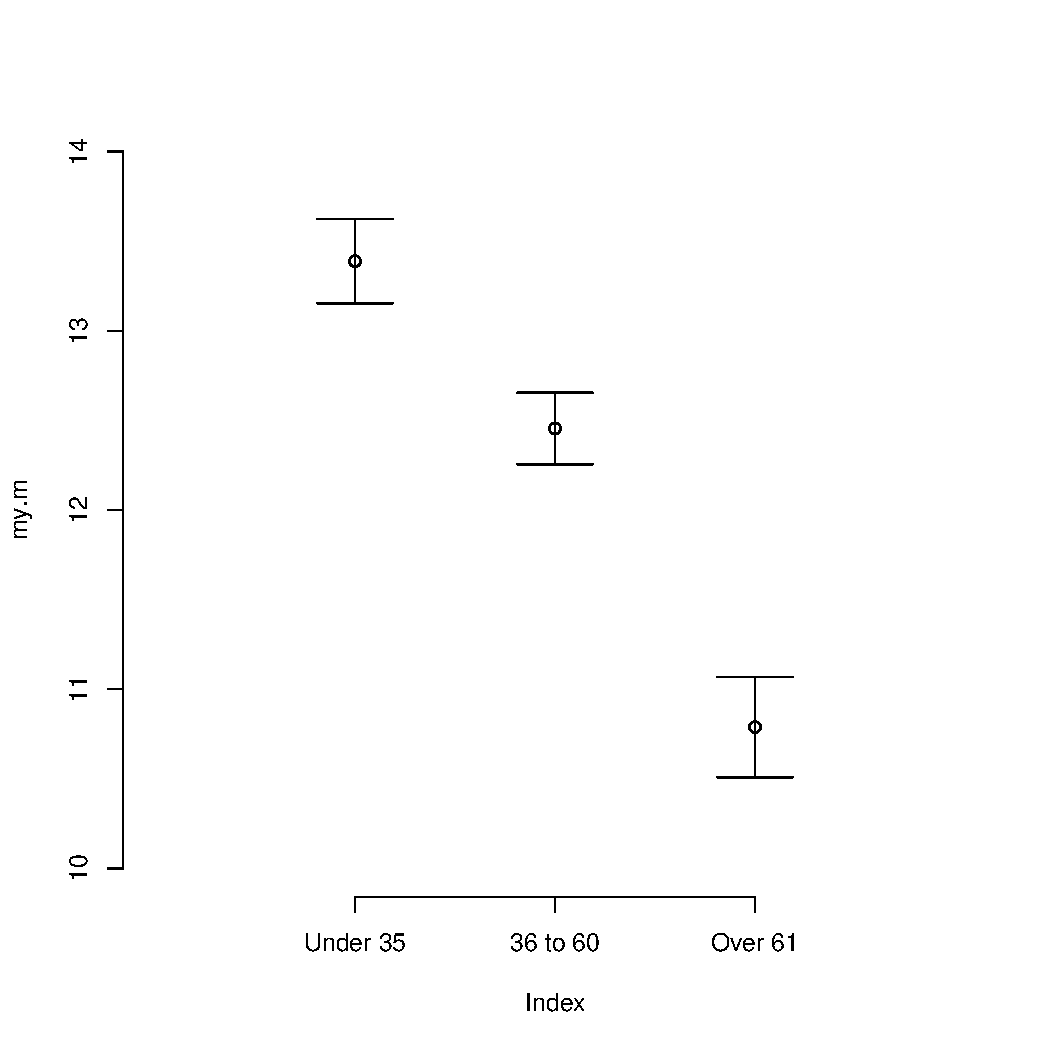
\includegraphics[height = 0.7\textwidth, keepaspectratio]{Figure/m4}
  %\vspace{-20pt}
  %\caption{Boxplots of PM10 in 2006--2012}
  \label{fig:m4}
\end{figure}
\end{frame} 

\begin{frame}[fragile]
  \frametitle{Essential embellishments}
\begin{itemize}
\item Need to draw an outer box that connects x-axis and y-axis.
\item The length of the heads of the error bars are too long.
\item Give correct labels for the axes 
\end{itemize}
\begin{knitrout}
\definecolor{shadecolor}{rgb}{0.965, 0.965, 0.965}\color{fgcolor}\begin{kframe}
\begin{alltt}
\hlkwd{plot}\hlstd{(my.m,} \hlkwc{ylim} \hlstd{=} \hlkwd{c}\hlstd{(}\hlnum{10}\hlstd{,} \hlnum{14}\hlstd{),} \hlkwc{xlim} \hlstd{=} \hlkwd{c}\hlstd{(}\hlnum{0}\hlstd{,} \hlnum{4}\hlstd{),} \hlkwc{axes} \hlstd{=} \hlnum{FALSE}\hlstd{,}
     \hlkwc{xlab} \hlstd{=} \hlstr{"Age group"}\hlstd{,}
     \hlkwc{ylab} \hlstd{=} \hlstr{"Mean total score"}\hlstd{)}
\hlkwd{arrows}\hlstd{(}\hlnum{1}\hlopt{:}\hlnum{3}\hlstd{, ci.lower,} \hlnum{1}\hlopt{:}\hlnum{3}\hlstd{, ci.upper,} \hlkwc{code} \hlstd{=} \hlnum{3}\hlstd{,}
       \hlkwc{length} \hlstd{=} \hlnum{.1}\hlstd{,} \hlkwc{angle} \hlstd{=} \hlnum{90}\hlstd{)}
\hlkwd{axis}\hlstd{(}\hlnum{2}\hlstd{)}
\hlkwd{axis}\hlstd{(}\hlnum{1}\hlstd{,} \hlkwc{at} \hlstd{=} \hlnum{1}\hlopt{:}\hlnum{3}\hlstd{,}
     \hlkwc{label} \hlstd{=} \hlkwd{c}\hlstd{(}\hlstr{"Under 35"}\hlstd{,} \hlstr{"36 to 60"}\hlstd{,} \hlstr{"Over 61"}\hlstd{))}
\hlkwd{box}\hlstd{()}
\end{alltt}
\end{kframe}
\end{knitrout}
\end{frame}


\begin{frame}[fragile]
  \frametitle{Essential embellishments}

\begin{figure}[h]
  \vspace{-20pt}
  \centering
  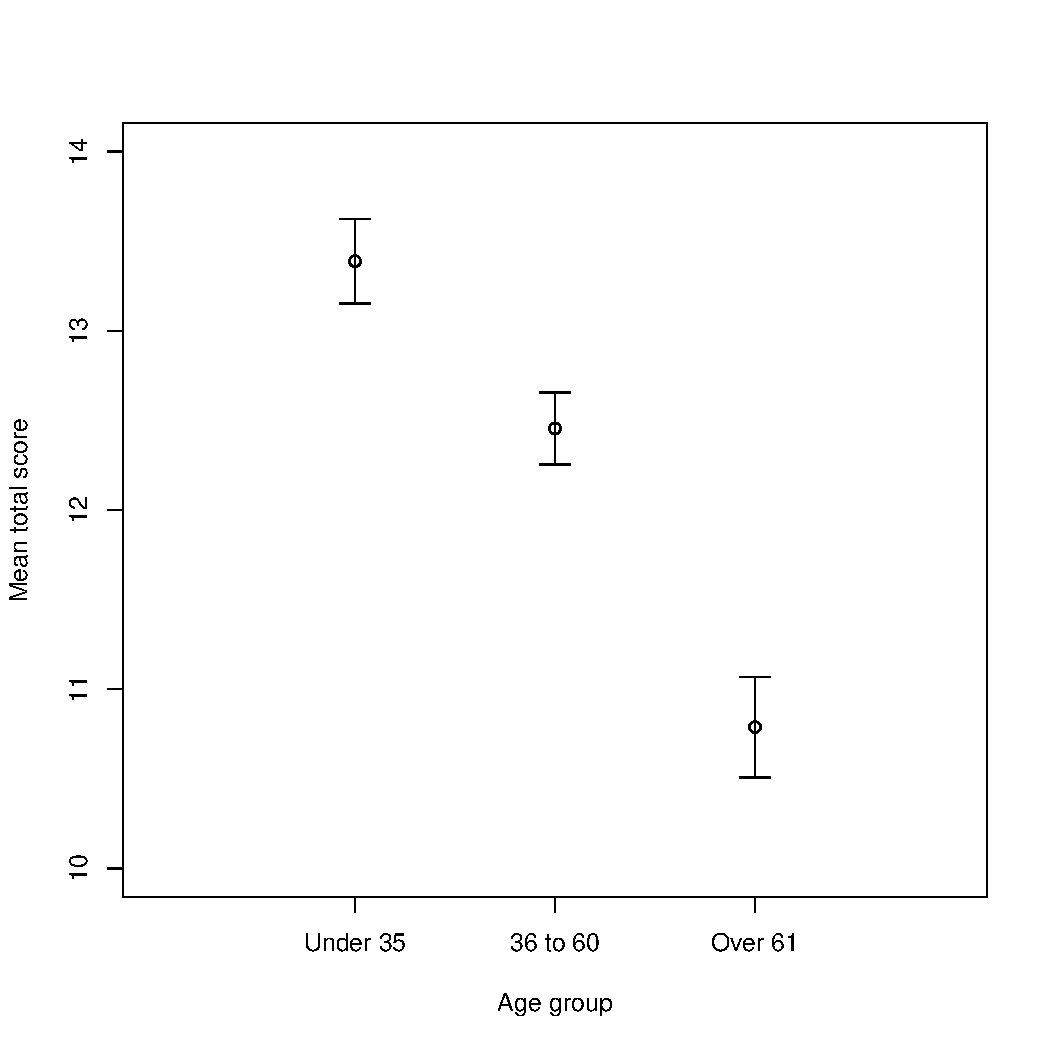
\includegraphics[height = 0.7\textwidth, keepaspectratio]{Figure/m5}
  %\vspace{-20pt}
  %\caption{Boxplots of PM10 in 2006--2012}
  \label{fig:m5}
\end{figure}
\end{frame} 



\begin{frame}[fragile]
  \frametitle{\texttt{ggplot2}}

\begin{figure}[h]
  \vspace{-20pt}
  \centering
  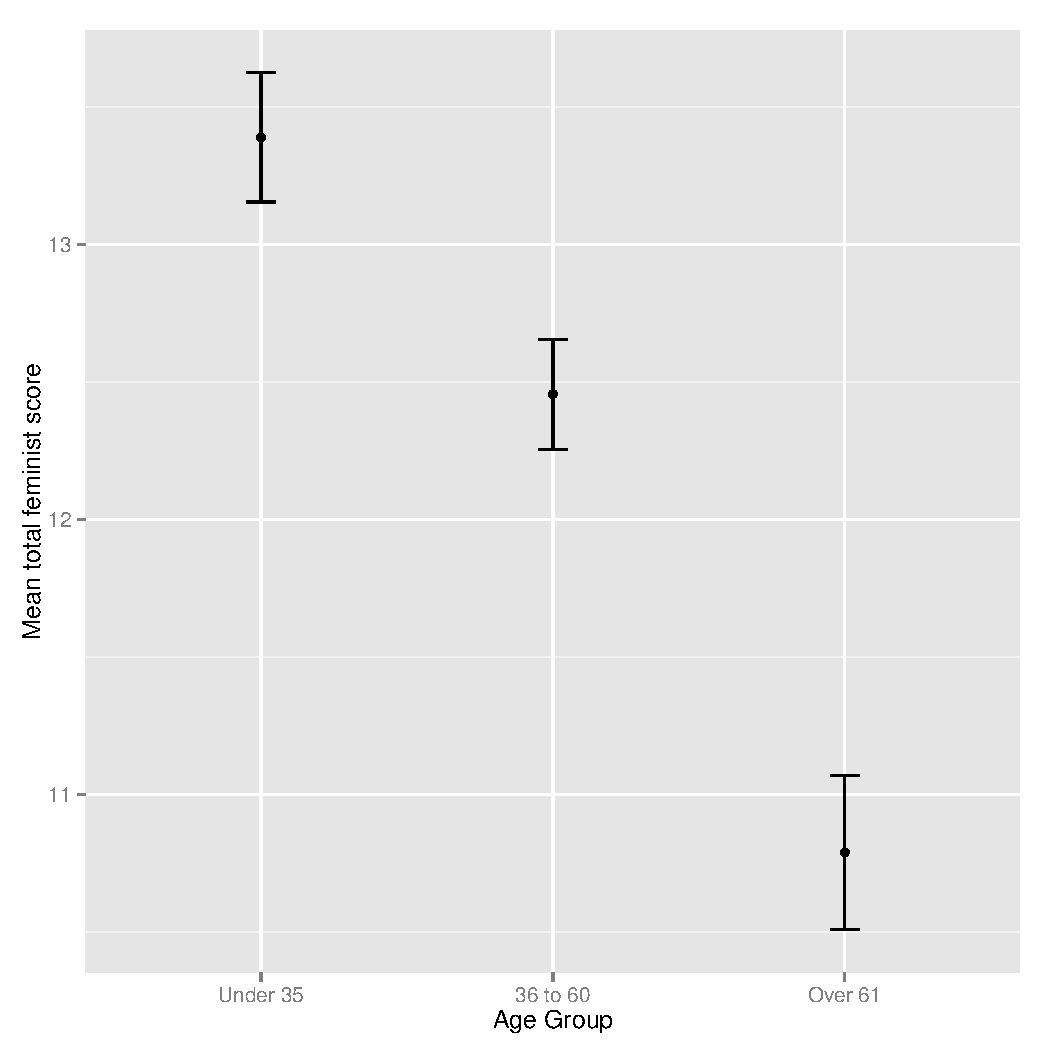
\includegraphics[height = 0.7\textwidth, keepaspectratio]{Figure/gg}
  %\vspace{-20pt}
  %\caption{Boxplots of PM10 in 2006--2012}
  \label{fig:gg}
\end{figure}
\end{frame} 
 
 
\begin{frame}[fragile]
  \frametitle{Any interactions between Gender and Age group?}
\begin{knitrout}
\definecolor{shadecolor}{rgb}{0.965, 0.965, 0.965}\color{fgcolor}\begin{kframe}
\begin{alltt}
\hlstd{GA.m} \hlkwb{<-} \hlkwd{with}\hlstd{(issp.df,} \hlkwd{tapply}\hlstd{(total.lik,}
           \hlkwd{list}\hlstd{(Gender, age.group), mean,} \hlkwc{na.rm} \hlstd{=} \hlnum{TRUE}\hlstd{))}
\hlstd{GA.m}
\end{alltt}
\begin{verbatim}
       Under 35 36 to 60  Over 61
Female  13.7500 12.64576 10.87234
Male    12.8963 12.16092 10.70526
\end{verbatim}
\end{kframe}
\end{knitrout}
We must plot these means in context. Therefore, we must calculate their corresponding (95\%) CIs.
\end{frame}


\begin{frame}[fragile]
  \frametitle{Calculating 95\% CIs}
\begin{knitrout}
\definecolor{shadecolor}{rgb}{0.965, 0.965, 0.965}\color{fgcolor}\begin{kframe}
\begin{alltt}
\hlstd{GA.sd} \hlkwb{<-} \hlkwd{with}\hlstd{(issp.df,} \hlkwd{tapply}\hlstd{(total.lik,}
              \hlkwd{list}\hlstd{(Gender, age.group), sd,} \hlkwc{na.rm} \hlstd{=} \hlnum{TRUE}\hlstd{))}
\hlstd{GA.n} \hlkwb{<-} \hlkwd{with}\hlstd{(issp.df,} \hlkwd{tapply}\hlstd{(total.lik,}
            \hlkwd{list}\hlstd{(Gender,age.group),}
            \hlkwa{function}\hlstd{(}\hlkwc{x}\hlstd{)}\hlkwd{length}\hlstd{(}\hlkwd{which}\hlstd{(}\hlopt{!}\hlkwd{is.na}\hlstd{(x)))))}
\hlstd{GA.stder} \hlkwb{<-} \hlstd{GA.sd}\hlopt{/}\hlkwd{sqrt}\hlstd{(GA.n)}
\hlstd{GA.upper} \hlkwb{<-} \hlstd{GA.m} \hlopt{+} \hlnum{1.96}\hlopt{*}\hlstd{GA.stder}
\hlstd{GA.lower} \hlkwb{<-} \hlstd{GA.m} \hlopt{-} \hlnum{1.96}\hlopt{*}\hlstd{GA.stder}
\hlstd{GA.lower}
\end{alltt}
\begin{verbatim}
       Under 35 36 to 60 Over 61
Female 13.44218 12.38896 10.5163
Male   12.54882 11.84390 10.2723
\end{verbatim}
\end{kframe}
\end{knitrout}
\end{frame} 


\begin{frame}[fragile]
  \frametitle{Step-by-step}
\begin{itemize}
\item The first (second) row of each of \texttt{GA.m}, \texttt{GA.lower}, \texttt{GA.upper} contains the mean, lower 95\% CI and upper 95\% CI, respectively, for female (male) respondents.
\item Plot the points and error bars (corresponding to lower/upper 95\% confidence limits) for females.
\item Repeat for males.
\end{itemize}
\begin{knitrout}
\definecolor{shadecolor}{rgb}{0.965, 0.965, 0.965}\color{fgcolor}\begin{kframe}
\begin{alltt}
\hlkwd{plot}\hlstd{(GA.m[}\hlnum{1}\hlstd{, ],} \hlkwc{xlab} \hlstd{=} \hlstr{"Age Group"}\hlstd{,}
     \hlkwc{ylab} \hlstd{=} \hlstr{"Mean feminist score"}\hlstd{,}
     \hlkwc{axes} \hlstd{=} \hlnum{FALSE}\hlstd{,} \hlkwc{xlim} \hlstd{=} \hlkwd{c}\hlstd{(}\hlnum{0}\hlstd{,} \hlnum{4}\hlstd{),} \hlkwc{ylim} \hlstd{=} \hlkwd{c}\hlstd{(}\hlnum{10}\hlstd{,} \hlnum{14.5}\hlstd{))}
\hlkwd{arrows}\hlstd{(}\hlnum{1}\hlopt{:}\hlnum{3}\hlstd{, GA.upper[}\hlnum{1}\hlstd{, ],} \hlnum{1}\hlopt{:}\hlnum{3}\hlstd{, GA.lower[}\hlnum{1}\hlstd{, ],}
       \hlkwc{angle} \hlstd{=} \hlnum{90}\hlstd{,} \hlkwc{code} \hlstd{=} \hlnum{3}\hlstd{,} \hlkwc{length} \hlstd{=} \hlnum{.1}\hlstd{)}
\hlkwd{axis}\hlstd{(}\hlnum{1}\hlstd{,} \hlkwc{at} \hlstd{=} \hlnum{1}\hlopt{:}\hlnum{3}\hlstd{,} \hlkwc{label} \hlstd{=} \hlkwd{colnames}\hlstd{(GA.m))}
\hlkwd{axis}\hlstd{(}\hlnum{2}\hlstd{)}
\hlkwd{box}\hlstd{()}
\end{alltt}
\end{kframe}
\end{knitrout}
\end{frame} 

\begin{frame}[fragile]
  \frametitle{Plotting mean $\pm$ 95\% CI: Females}

\begin{figure}[h]
  \vspace{-20pt}
  \centering
  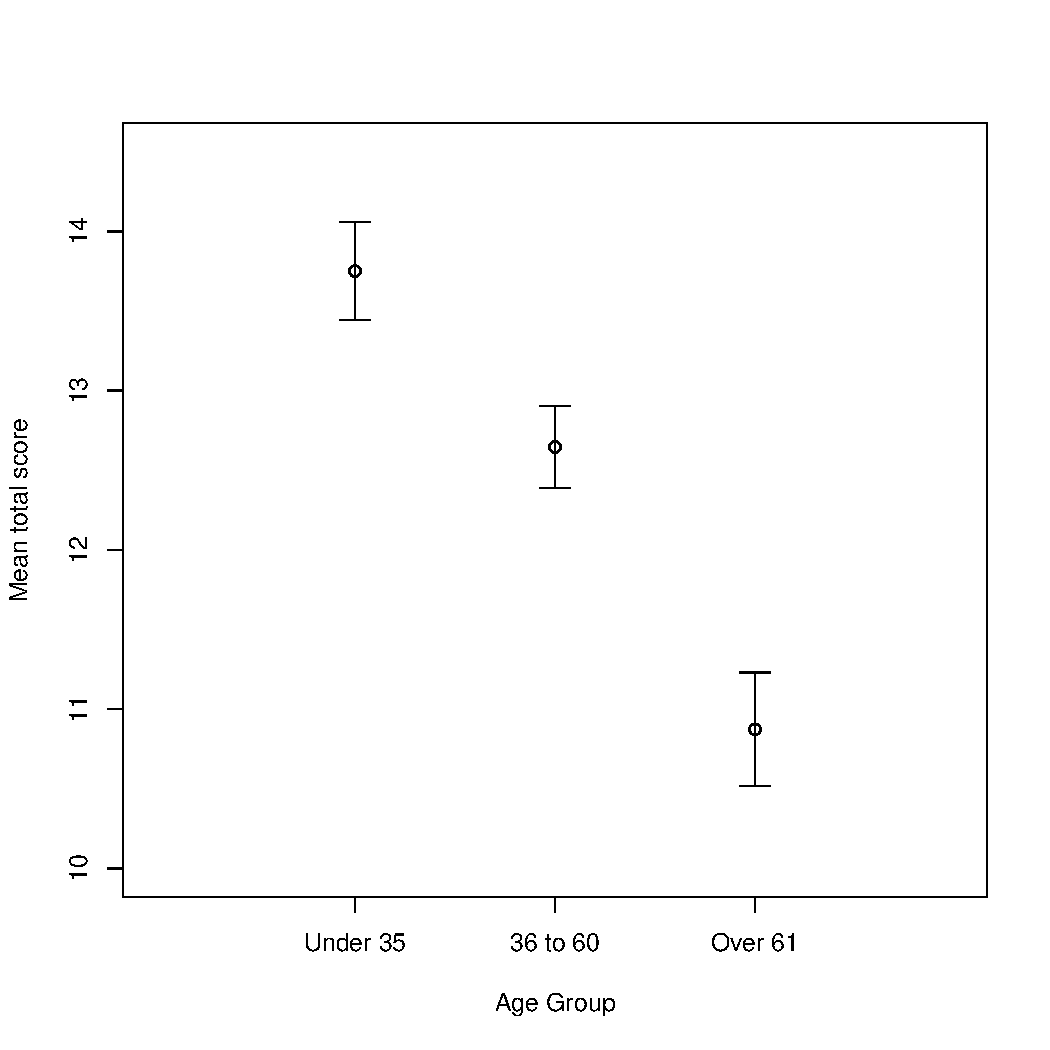
\includegraphics[height = 0.7\textwidth, keepaspectratio]{Figure/m6}
  %\vspace{-20pt}
  %\caption{Boxplots of PM10 in 2006--2012}
  \label{fig:m6}
\end{figure}
\end{frame} 


\begin{frame}[fragile]
  \frametitle{Plotting mean $\pm$ 95\% CI: Males}
Using \textcolor{blue}{blue} symbols/lines for males.
\begin{knitrout}
\definecolor{shadecolor}{rgb}{0.965, 0.965, 0.965}\color{fgcolor}\begin{kframe}
\begin{alltt}
\hlkwd{plot}\hlstd{(GA.m[}\hlnum{1}\hlstd{, ],} \hlkwc{xlab} \hlstd{=} \hlstr{"Age Group"}\hlstd{,}
     \hlkwc{ylab} \hlstd{=} \hlstr{"Mean total score"}\hlstd{,}
     \hlkwc{axes} \hlstd{=} \hlnum{FALSE}\hlstd{,} \hlkwc{xlim} \hlstd{=} \hlkwd{c}\hlstd{(}\hlnum{0}\hlstd{,} \hlnum{4}\hlstd{),} \hlkwc{ylim} \hlstd{=} \hlkwd{c}\hlstd{(}\hlnum{10}\hlstd{,} \hlnum{14.5}\hlstd{))}
\hlkwd{arrows}\hlstd{(}\hlnum{1}\hlopt{:}\hlnum{3}\hlstd{, GA.upper[}\hlnum{1}\hlstd{, ],} \hlnum{1}\hlopt{:}\hlnum{3}\hlstd{, GA.lower[}\hlnum{1}\hlstd{, ],}
       \hlkwc{angle} \hlstd{=} \hlnum{90}\hlstd{,} \hlkwc{code} \hlstd{=} \hlnum{3}\hlstd{,} \hlkwc{length} \hlstd{=} \hlnum{.1}\hlstd{)}
\hlkwd{axis}\hlstd{(}\hlnum{1}\hlstd{,} \hlkwc{at} \hlstd{=} \hlnum{1}\hlopt{:}\hlnum{3}\hlstd{,} \hlkwc{label} \hlstd{=} \hlkwd{colnames}\hlstd{(GA.m))}
\hlkwd{axis}\hlstd{(}\hlnum{2}\hlstd{)}
\hlkwd{box}\hlstd{()}
\hlkwd{points}\hlstd{(GA.m[}\hlnum{2}\hlstd{, ],} \hlkwc{col} \hlstd{=} \hlstr{"blue"}\hlstd{)}
\hlkwd{arrows}\hlstd{(}\hlnum{1}\hlopt{:}\hlnum{3}\hlstd{, GA.upper[}\hlnum{2}\hlstd{, ],} \hlnum{1}\hlopt{:}\hlnum{3}\hlstd{, GA.lower[}\hlnum{2}\hlstd{, ],}
       \hlkwc{angle} \hlstd{=} \hlnum{90}\hlstd{,} \hlkwc{code} \hlstd{=} \hlnum{3}\hlstd{,} \hlkwc{length} \hlstd{=} \hlnum{.1}\hlstd{,} \hlkwc{col} \hlstd{=} \hlstr{"blue"}\hlstd{)}
\end{alltt}
\end{kframe}
\end{knitrout}
\end{frame} 

\begin{frame}[fragile]
  \frametitle{Add the means for males}

\begin{figure}[h]
  \vspace{-20pt}
  \centering
  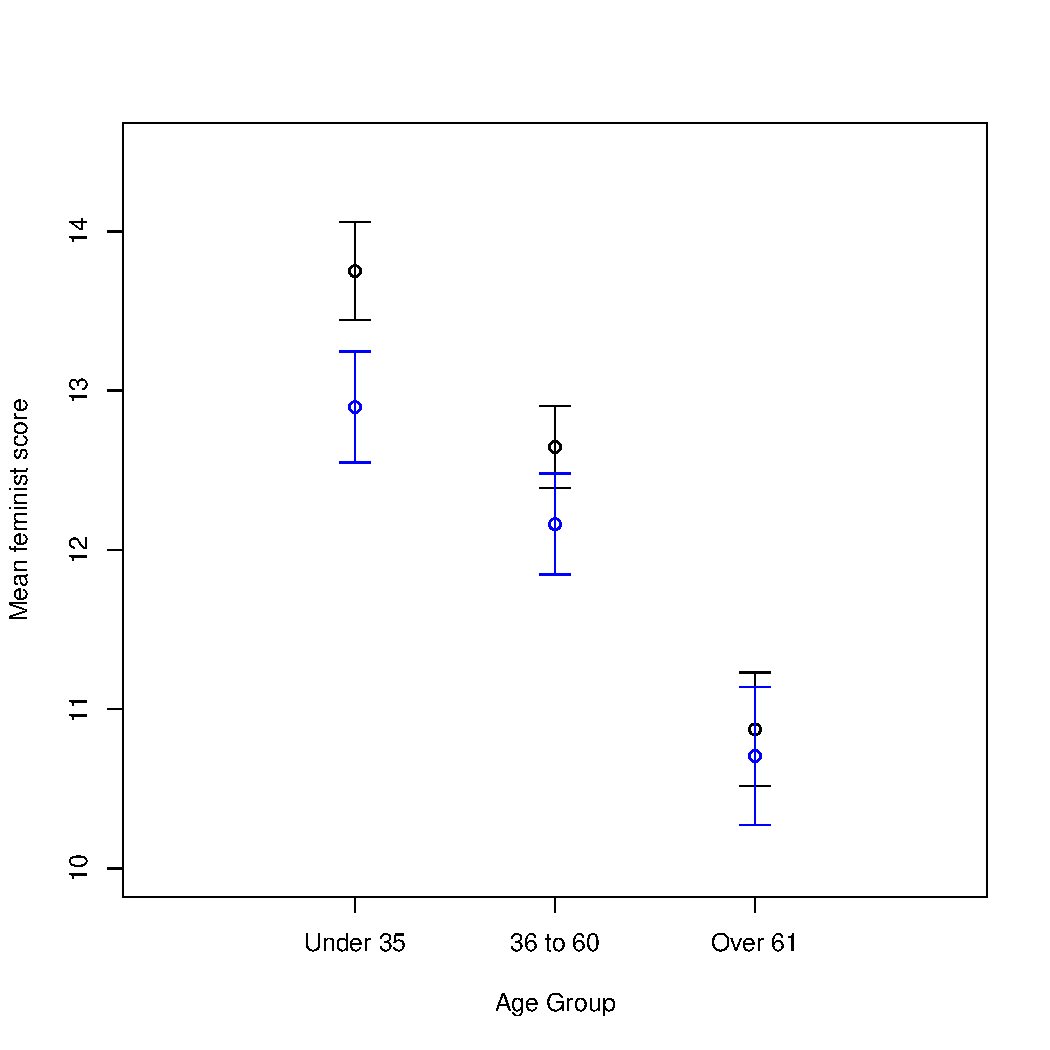
\includegraphics[height = 0.7\textwidth, keepaspectratio]{Figure/m7}
  %\vspace{-20pt}
  %\caption{Boxplots of PM10 in 2006--2012}
  \label{fig:m7}
\end{figure}
\end{frame} 

\begin{frame}
\frametitle{Improvements}
\begin{itemize}
\item Points/error bars overlay one another. Need to separate them?
\item So far, we have plotted means/error bars at x = 1, 2 and 3. We can use different x coordinates for males and females.
\item Probably the space between age groups should be larger than the space between males and females.
\item How about:
  \begin{itemize}
    \item Female: x = 1, 3, 5.
    \item Male: x = 1.5, 3.5, 5.5
  \end{itemize}
\end{itemize}
\end{frame}


\begin{frame}[fragile]
  \frametitle{Side-by-side}
\begin{knitrout}
\definecolor{shadecolor}{rgb}{0.965, 0.965, 0.965}\color{fgcolor}\begin{kframe}
\begin{alltt}
\hlkwd{plot}\hlstd{(}\hlkwd{c}\hlstd{(}\hlnum{1}\hlstd{,} \hlnum{3}\hlstd{,} \hlnum{5}\hlstd{), GA.m[}\hlnum{1}\hlstd{, ],} \hlkwc{xlab} \hlstd{=} \hlstr{"Age Group"}\hlstd{,}
     \hlkwc{ylab} \hlstd{=} \hlstr{"Mean feminist score"}\hlstd{,}\hlkwc{col} \hlstd{=} \hlnum{1}\hlstd{,}
     \hlkwc{axes} \hlstd{=} \hlnum{FALSE}\hlstd{,} \hlkwc{xlim} \hlstd{=} \hlkwd{c}\hlstd{(}\hlnum{0}\hlstd{,} \hlnum{6.5}\hlstd{),} \hlkwc{ylim} \hlstd{=} \hlkwd{c}\hlstd{(}\hlnum{10}\hlstd{,} \hlnum{14.5}\hlstd{))}
\hlkwd{arrows}\hlstd{(}\hlkwd{c}\hlstd{(}\hlnum{1}\hlstd{,} \hlnum{3}\hlstd{,} \hlnum{5}\hlstd{), GA.upper[}\hlnum{1}\hlstd{, ],} \hlkwd{c}\hlstd{(}\hlnum{1}\hlstd{,} \hlnum{3}\hlstd{,} \hlnum{5}\hlstd{),}
       \hlstd{GA.lower[}\hlnum{1}\hlstd{, ],}
       \hlkwc{angle} \hlstd{=} \hlnum{90}\hlstd{,} \hlkwc{code} \hlstd{=} \hlnum{3}\hlstd{,} \hlkwc{length} \hlstd{=} \hlnum{.1}\hlstd{,} \hlkwc{col} \hlstd{=} \hlnum{1}\hlstd{)}
\hlkwd{points}\hlstd{(}\hlkwd{c}\hlstd{(}\hlnum{1.5}\hlstd{,} \hlnum{3.5}\hlstd{,} \hlnum{5.5}\hlstd{),GA.m[}\hlnum{2}\hlstd{, ],} \hlkwc{col} \hlstd{=} \hlstr{"blue"}\hlstd{)}
\hlkwd{arrows}\hlstd{(}\hlkwd{c}\hlstd{(}\hlnum{1.5}\hlstd{,} \hlnum{3.5}\hlstd{,} \hlnum{5.5}\hlstd{), GA.upper[}\hlnum{2}\hlstd{, ],} \hlkwd{c}\hlstd{(}\hlnum{1.5}\hlstd{,} \hlnum{3.5}\hlstd{,} \hlnum{5.5}\hlstd{),}
       \hlstd{GA.lower[}\hlnum{2}\hlstd{, ],}
       \hlkwc{angle} \hlstd{=} \hlnum{90}\hlstd{,} \hlkwc{code} \hlstd{=} \hlnum{3}\hlstd{,} \hlkwc{length} \hlstd{=} \hlnum{.1}\hlstd{,} \hlkwc{col} \hlstd{=} \hlstr{"blue"}\hlstd{)}
\hlkwd{axis}\hlstd{(}\hlnum{1}\hlstd{)}
\end{alltt}
\end{kframe}
\end{knitrout}
\end{frame} 

\begin{frame}[fragile]
  \frametitle{Side-by-side}

\begin{figure}[h]
  \vspace{-20pt}
  \centering
  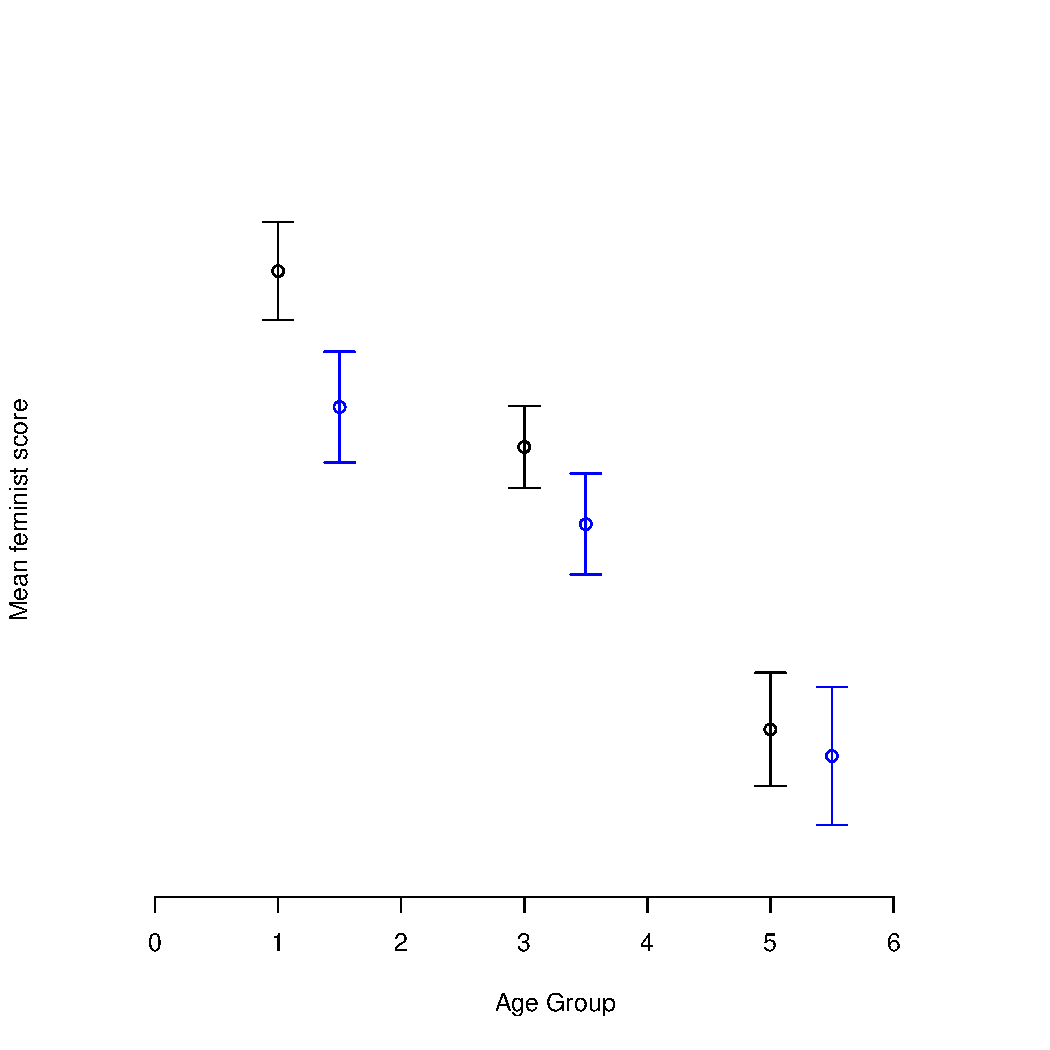
\includegraphics[height = 0.7\textwidth, keepaspectratio]{Figure/m8}
  %\vspace{-20pt}
  %\caption{Boxplots of PM10 in 2006--2012}
  \label{fig:m8}
\end{figure}
\end{frame} 


\begin{frame}[fragile]
  \frametitle{Tidy up tick marks and labels on x-axis}
\begin{knitrout}
\definecolor{shadecolor}{rgb}{0.965, 0.965, 0.965}\color{fgcolor}\begin{kframe}
\begin{alltt}
\hlkwd{plot}\hlstd{(}\hlkwd{c}\hlstd{(}\hlnum{1}\hlstd{,} \hlnum{3}\hlstd{,} \hlnum{5}\hlstd{), GA.m[}\hlnum{1}\hlstd{, ],} \hlkwc{xlab} \hlstd{=} \hlstr{"Age Group"}\hlstd{,}
     \hlkwc{ylab} \hlstd{=} \hlstr{"Mean feminist score"}\hlstd{,}\hlkwc{col} \hlstd{=} \hlnum{1}\hlstd{,}
     \hlkwc{axes} \hlstd{=} \hlnum{FALSE}\hlstd{,} \hlkwc{xlim} \hlstd{=} \hlkwd{c}\hlstd{(}\hlnum{0}\hlstd{,} \hlnum{6.5}\hlstd{),} \hlkwc{ylim} \hlstd{=} \hlkwd{c}\hlstd{(}\hlnum{10}\hlstd{,} \hlnum{14.5}\hlstd{))}
\hlkwd{arrows}\hlstd{(}\hlkwd{c}\hlstd{(}\hlnum{1}\hlstd{,} \hlnum{3}\hlstd{,} \hlnum{5}\hlstd{), GA.upper[}\hlnum{1}\hlstd{, ],} \hlkwd{c}\hlstd{(}\hlnum{1}\hlstd{,} \hlnum{3}\hlstd{,} \hlnum{5}\hlstd{),}
       \hlstd{GA.lower[}\hlnum{1}\hlstd{, ],}
       \hlkwc{angle} \hlstd{=} \hlnum{90}\hlstd{,} \hlkwc{code} \hlstd{=} \hlnum{3}\hlstd{,} \hlkwc{length} \hlstd{=} \hlnum{.1}\hlstd{,} \hlkwc{col} \hlstd{=} \hlnum{1}\hlstd{)}
\hlkwd{points}\hlstd{(}\hlkwd{c}\hlstd{(}\hlnum{1.5}\hlstd{,} \hlnum{3.5}\hlstd{,} \hlnum{5.5}\hlstd{),GA.m[}\hlnum{2}\hlstd{, ],} \hlkwc{col} \hlstd{=} \hlstr{"blue"}\hlstd{)}
\hlkwd{arrows}\hlstd{(}\hlkwd{c}\hlstd{(}\hlnum{1.5}\hlstd{,} \hlnum{3.5}\hlstd{,} \hlnum{5.5}\hlstd{), GA.upper[}\hlnum{2}\hlstd{, ],} \hlkwd{c}\hlstd{(}\hlnum{1.5}\hlstd{,} \hlnum{3.5}\hlstd{,} \hlnum{5.5}\hlstd{),}
       \hlstd{GA.lower[}\hlnum{2}\hlstd{, ],}
       \hlkwc{angle} \hlstd{=} \hlnum{90}\hlstd{,} \hlkwc{code} \hlstd{=} \hlnum{3}\hlstd{,} \hlkwc{length} \hlstd{=} \hlnum{.1}\hlstd{,} \hlkwc{col} \hlstd{=} \hlstr{"blue"}\hlstd{)}
\hlkwd{axis}\hlstd{(}\hlnum{1}\hlstd{,} \hlkwc{at} \hlstd{=} \hlkwd{c}\hlstd{(}\hlnum{1.25}\hlstd{,} \hlnum{3.25}\hlstd{,} \hlnum{5.25}\hlstd{),} \hlkwc{label} \hlstd{=} \hlkwd{colnames}\hlstd{(GA.m))}
\hlkwd{axis}\hlstd{(}\hlnum{2}\hlstd{)}
\hlkwd{box}\hlstd{()}
\end{alltt}
\end{kframe}
\end{knitrout}
\end{frame} 

\begin{frame}[fragile]
  \frametitle{Add a box around the figure}

\begin{figure}[h]
  \vspace{-20pt}
  \centering
  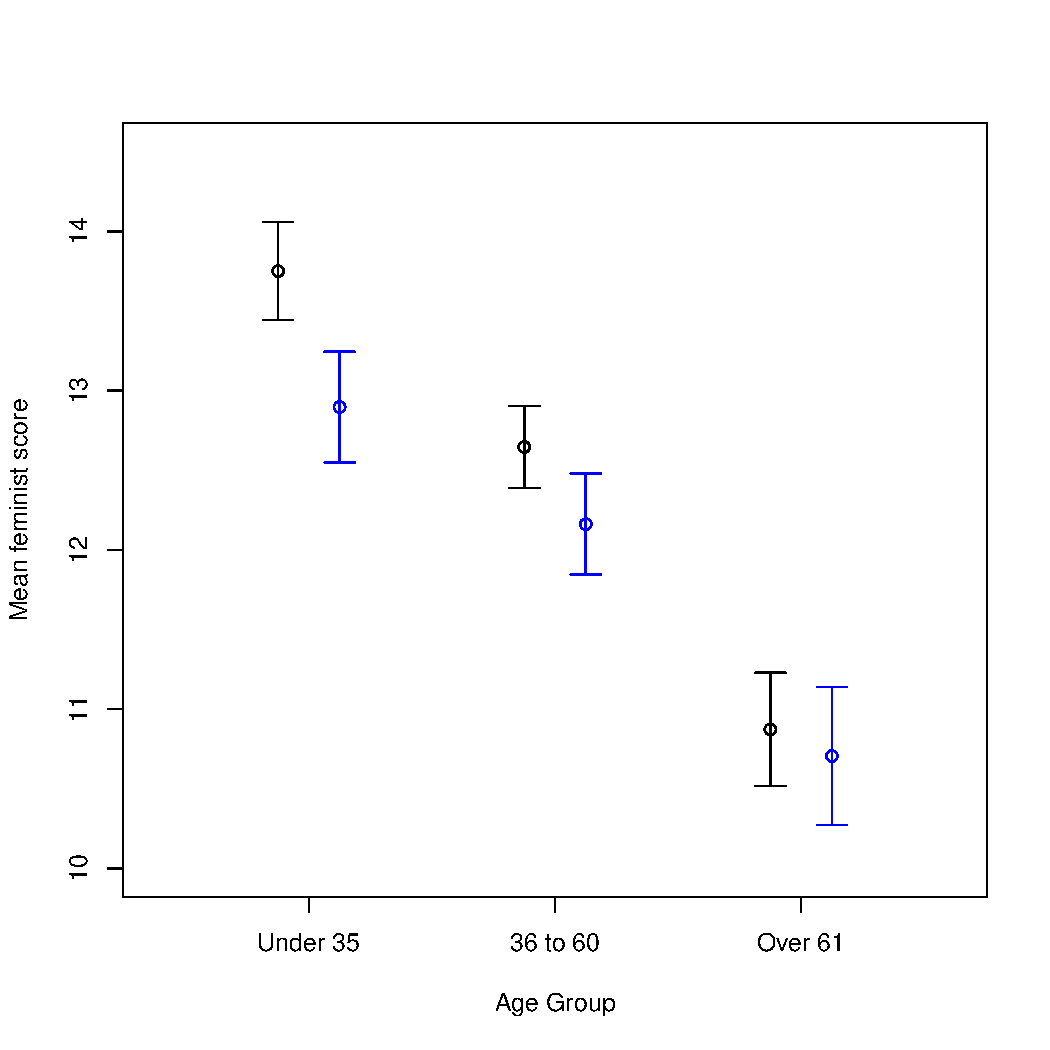
\includegraphics[height = 0.7\textwidth, keepaspectratio]{Figure/m9}
  %\vspace{-20pt}
  %\caption{Boxplots of PM10 in 2006--2012}
  \label{fig:m9}
\end{figure}
\end{frame} 


\begin{frame}[fragile]
  \frametitle{Connect the points?}
\begin{knitrout}
\definecolor{shadecolor}{rgb}{0.965, 0.965, 0.965}\color{fgcolor}\begin{kframe}
\begin{alltt}
\hlkwd{plot}\hlstd{(}\hlkwd{c}\hlstd{(}\hlnum{1}\hlstd{,} \hlnum{3}\hlstd{,} \hlnum{5}\hlstd{), GA.m[}\hlnum{1}\hlstd{, ],} \hlkwc{xlab} \hlstd{=} \hlstr{"Age Group"}\hlstd{,}
     \hlkwc{ylab} \hlstd{=} \hlstr{"Mean feminist score"}\hlstd{,}\hlkwc{col} \hlstd{=} \hlnum{1}\hlstd{,} \hlkwc{type} \hlstd{=} \hlstr{"b"}\hlstd{,}
     \hlkwc{axes} \hlstd{=} \hlnum{FALSE}\hlstd{,} \hlkwc{xlim} \hlstd{=} \hlkwd{c}\hlstd{(}\hlnum{0}\hlstd{,} \hlnum{6.5}\hlstd{),} \hlkwc{ylim} \hlstd{=} \hlkwd{c}\hlstd{(}\hlnum{10}\hlstd{,} \hlnum{14.5}\hlstd{))}
\hlkwd{arrows}\hlstd{(}\hlkwd{c}\hlstd{(}\hlnum{1}\hlstd{,} \hlnum{3}\hlstd{,} \hlnum{5}\hlstd{), GA.upper[}\hlnum{1}\hlstd{, ],} \hlkwd{c}\hlstd{(}\hlnum{1}\hlstd{,} \hlnum{3}\hlstd{,} \hlnum{5}\hlstd{),}
       \hlstd{GA.lower[}\hlnum{1}\hlstd{, ],}
       \hlkwc{angle} \hlstd{=} \hlnum{90}\hlstd{,} \hlkwc{code} \hlstd{=} \hlnum{3}\hlstd{,} \hlkwc{length} \hlstd{=} \hlnum{.1}\hlstd{,} \hlkwc{col} \hlstd{=} \hlnum{1}\hlstd{)}
\hlkwd{points}\hlstd{(}\hlkwd{c}\hlstd{(}\hlnum{1.5}\hlstd{,} \hlnum{3.5}\hlstd{,} \hlnum{5.5}\hlstd{),GA.m[}\hlnum{2}\hlstd{, ],} \hlkwc{col} \hlstd{=} \hlstr{"blue"}\hlstd{,} \hlkwc{type} \hlstd{=} \hlstr{"b"}\hlstd{)}
\hlkwd{arrows}\hlstd{(}\hlkwd{c}\hlstd{(}\hlnum{1.5}\hlstd{,} \hlnum{3.5}\hlstd{,} \hlnum{5.5}\hlstd{), GA.upper[}\hlnum{2}\hlstd{, ],} \hlkwd{c}\hlstd{(}\hlnum{1.5}\hlstd{,} \hlnum{3.5}\hlstd{,} \hlnum{5.5}\hlstd{),}
       \hlstd{GA.lower[}\hlnum{2}\hlstd{, ],}
       \hlkwc{angle} \hlstd{=} \hlnum{90}\hlstd{,} \hlkwc{code} \hlstd{=} \hlnum{3}\hlstd{,} \hlkwc{length} \hlstd{=} \hlnum{.1}\hlstd{,} \hlkwc{col} \hlstd{=} \hlstr{"blue"}\hlstd{)}
\hlkwd{axis}\hlstd{(}\hlnum{1}\hlstd{,} \hlkwc{at} \hlstd{=} \hlkwd{c}\hlstd{(}\hlnum{1.25}\hlstd{,} \hlnum{3.25}\hlstd{,} \hlnum{5.25}\hlstd{),} \hlkwc{label} \hlstd{=} \hlkwd{colnames}\hlstd{(GA.m))}
\hlkwd{axis}\hlstd{(}\hlnum{2}\hlstd{)}
\hlkwd{box}\hlstd{()}
\end{alltt}
\end{kframe}
\end{knitrout}
\end{frame} 

\begin{frame}[fragile]
  \frametitle{Connect the points}

\begin{figure}[h]
  \vspace{-20pt}
  \centering
  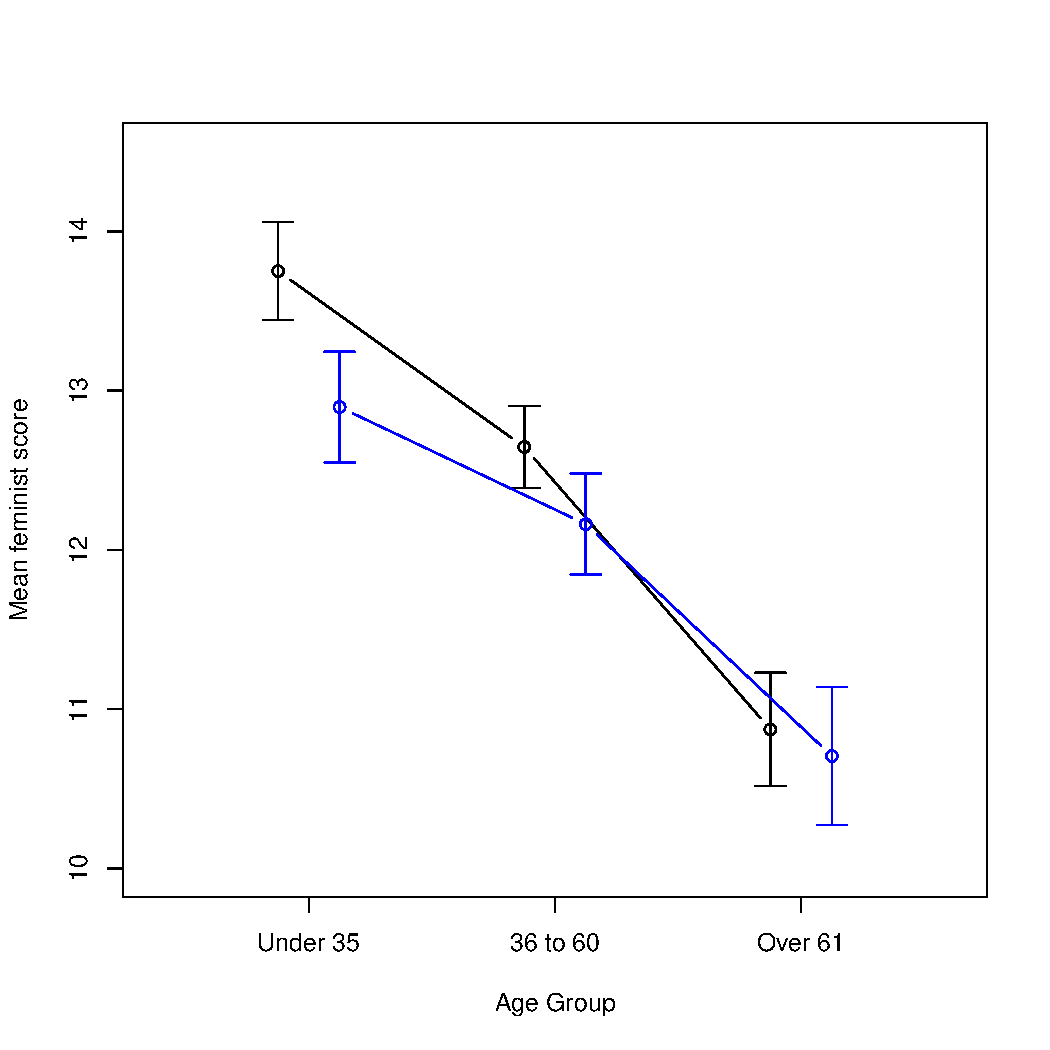
\includegraphics[height = 0.7\textwidth, keepaspectratio]{Figure/m10}
  %\vspace{-20pt}
  %\caption{Boxplots of PM10 in 2006--2012}
  \label{fig:m10}
\end{figure}
\end{frame} 


\begin{frame}[fragile]
  \frametitle{Add legend}
\begin{knitrout}
\definecolor{shadecolor}{rgb}{0.965, 0.965, 0.965}\color{fgcolor}\begin{kframe}
\begin{alltt}
\hlkwd{plot}\hlstd{(}\hlkwd{c}\hlstd{(}\hlnum{1}\hlstd{,} \hlnum{3}\hlstd{,} \hlnum{5}\hlstd{), GA.m[}\hlnum{1}\hlstd{, ],} \hlkwc{xlab} \hlstd{=} \hlstr{"Age Group"}\hlstd{,}
     \hlkwc{ylab} \hlstd{=} \hlstr{"Mean feminist score"}\hlstd{,}\hlkwc{col} \hlstd{=} \hlnum{1}\hlstd{,} \hlkwc{type} \hlstd{=} \hlstr{"b"}\hlstd{,}
     \hlkwc{axes} \hlstd{=} \hlnum{FALSE}\hlstd{,} \hlkwc{xlim} \hlstd{=} \hlkwd{c}\hlstd{(}\hlnum{0}\hlstd{,} \hlnum{6.5}\hlstd{),} \hlkwc{ylim} \hlstd{=} \hlkwd{c}\hlstd{(}\hlnum{10}\hlstd{,} \hlnum{14.5}\hlstd{))}
\hlkwd{arrows}\hlstd{(}\hlkwd{c}\hlstd{(}\hlnum{1}\hlstd{,} \hlnum{3}\hlstd{,} \hlnum{5}\hlstd{), GA.upper[}\hlnum{1}\hlstd{, ],} \hlkwd{c}\hlstd{(}\hlnum{1}\hlstd{,} \hlnum{3}\hlstd{,} \hlnum{5}\hlstd{),}
       \hlstd{GA.lower[}\hlnum{1}\hlstd{, ],}
       \hlkwc{angle} \hlstd{=} \hlnum{90}\hlstd{,} \hlkwc{code} \hlstd{=} \hlnum{3}\hlstd{,} \hlkwc{length} \hlstd{=} \hlnum{.1}\hlstd{,} \hlkwc{col} \hlstd{=} \hlnum{1}\hlstd{)}
\hlkwd{points}\hlstd{(}\hlkwd{c}\hlstd{(}\hlnum{1.5}\hlstd{,} \hlnum{3.5}\hlstd{,} \hlnum{5.5}\hlstd{),GA.m[}\hlnum{2}\hlstd{, ],} \hlkwc{col} \hlstd{=} \hlstr{"blue"}\hlstd{,} \hlkwc{type} \hlstd{=} \hlstr{"b"}\hlstd{)}
\hlkwd{arrows}\hlstd{(}\hlkwd{c}\hlstd{(}\hlnum{1.5}\hlstd{,} \hlnum{3.5}\hlstd{,} \hlnum{5.5}\hlstd{), GA.upper[}\hlnum{2}\hlstd{, ],} \hlkwd{c}\hlstd{(}\hlnum{1.5}\hlstd{,} \hlnum{3.5}\hlstd{,} \hlnum{5.5}\hlstd{),}
       \hlstd{GA.lower[}\hlnum{2}\hlstd{, ],}
       \hlkwc{angle} \hlstd{=} \hlnum{90}\hlstd{,} \hlkwc{code} \hlstd{=} \hlnum{3}\hlstd{,} \hlkwc{length} \hlstd{=} \hlnum{.1}\hlstd{,} \hlkwc{col} \hlstd{=} \hlstr{"blue"}\hlstd{)}
\hlkwd{axis}\hlstd{(}\hlnum{1}\hlstd{,} \hlkwc{at} \hlstd{=} \hlkwd{c}\hlstd{(}\hlnum{1.25}\hlstd{,} \hlnum{3.25}\hlstd{,} \hlnum{5.25}\hlstd{),} \hlkwc{label} \hlstd{=} \hlkwd{colnames}\hlstd{(GA.m))}
\hlkwd{axis}\hlstd{(}\hlnum{2}\hlstd{)}
\hlkwd{box}\hlstd{()}
\hlkwd{legend}\hlstd{(}\hlstr{"topright"}\hlstd{,} \hlkwc{pch} \hlstd{=} \hlnum{21}\hlstd{,} \hlkwc{lty} \hlstd{=} \hlnum{1}\hlstd{,} \hlkwc{bty} \hlstd{=} \hlstr{"n"}\hlstd{,}
       \hlkwc{col} \hlstd{=} \hlkwd{c}\hlstd{(}\hlstr{"black"}\hlstd{,} \hlstr{"blue"}\hlstd{),} \hlkwc{cex} \hlstd{=} \hlnum{1.5}\hlstd{,}
       \hlkwc{legend} \hlstd{=} \hlkwd{c}\hlstd{(}\hlstr{"Female"}\hlstd{,} \hlstr{"Male"}\hlstd{))}
\end{alltt}
\end{kframe}
\end{knitrout}
\end{frame} 

\begin{frame}[fragile]
  \frametitle{Add legend}

\begin{figure}[h]
  \vspace{-20pt}
  \centering
  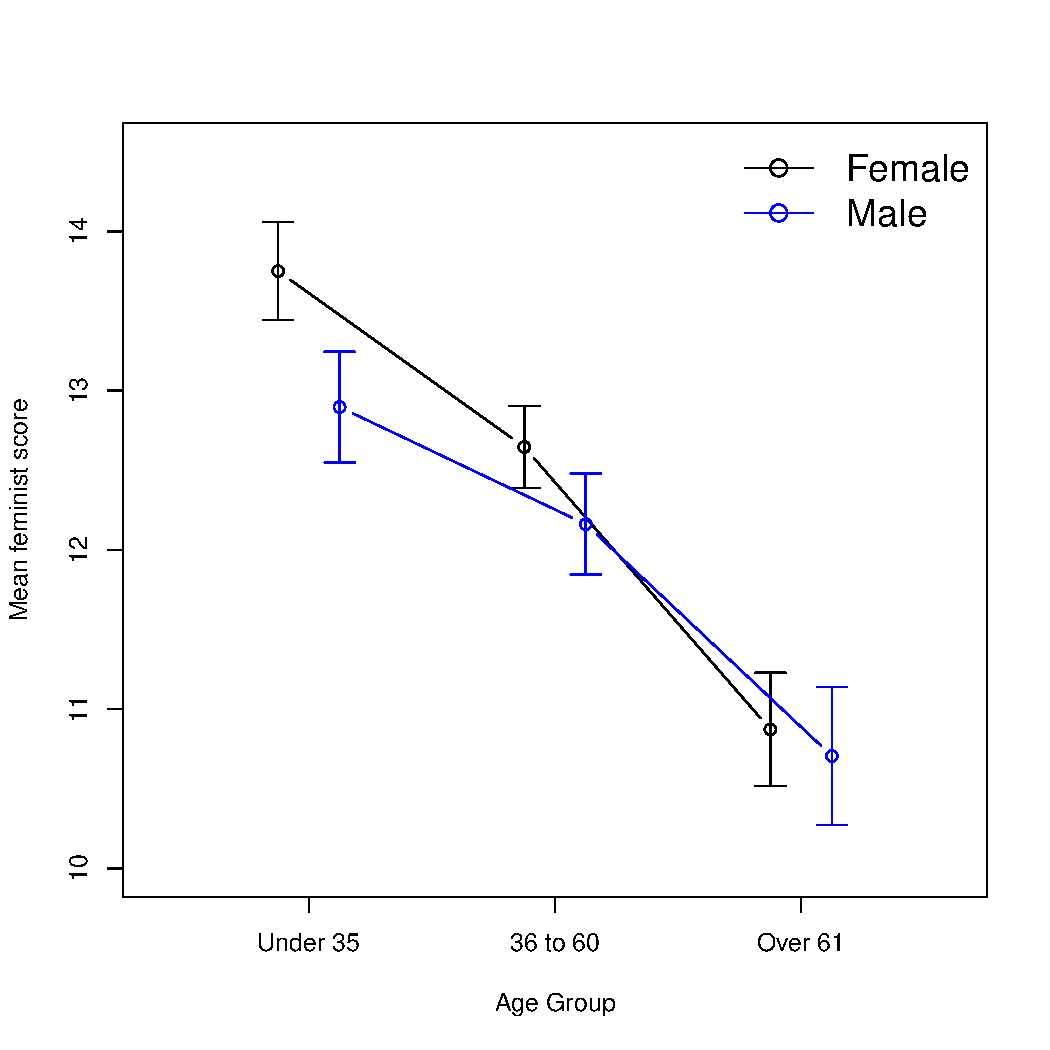
\includegraphics[height = 0.7\textwidth, keepaspectratio]{Figure/m11}
  %\vspace{-20pt}
  %\caption{Boxplots of PM10 in 2006--2012}
  \label{fig:m11}
\end{figure}
\end{frame}



\begin{frame}[fragile]
  \frametitle{\texttt{ggplot2}}

\begin{figure}[h]
  \vspace{-20pt}
  \centering
  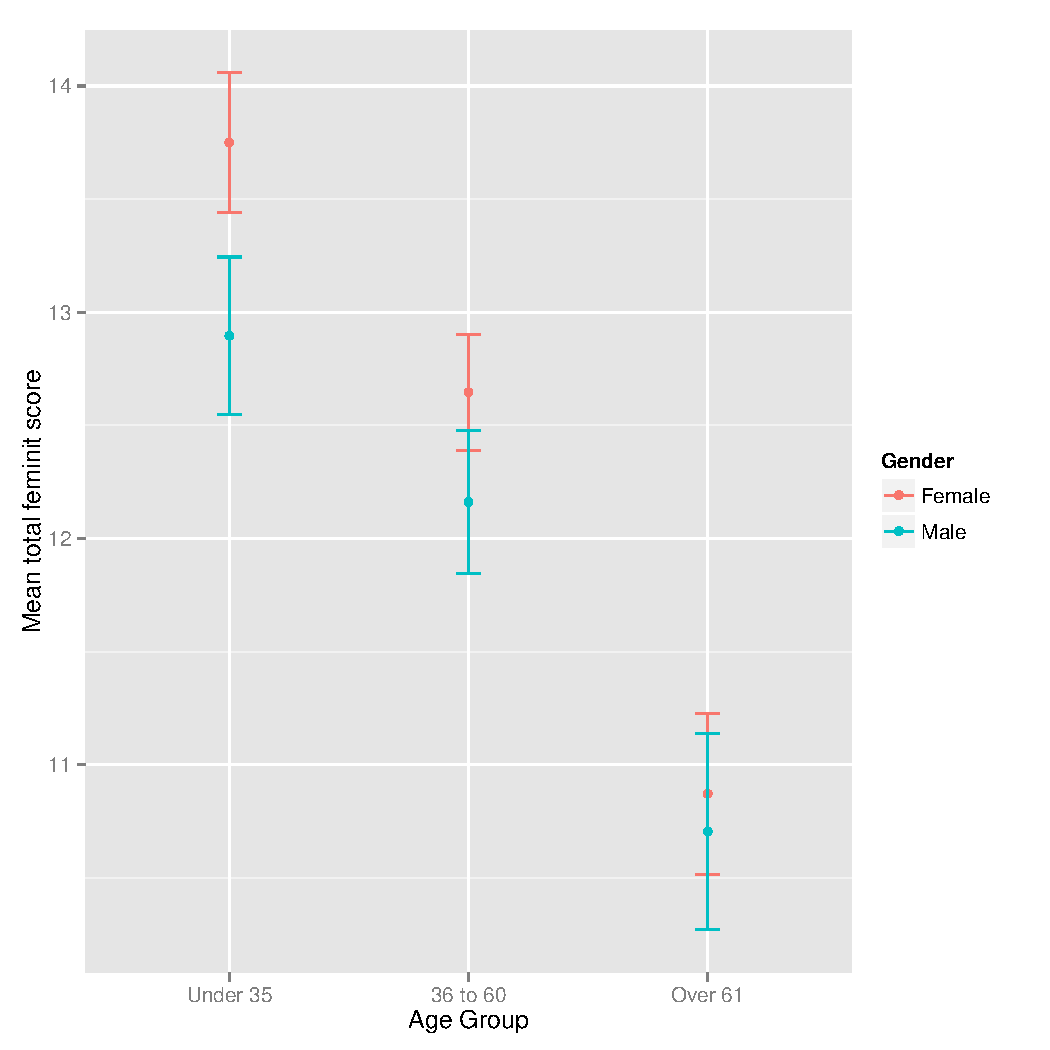
\includegraphics[height = 0.7\textwidth, keepaspectratio]{Figure/gg1}
  %\vspace{-20pt}
  %\caption{Boxplots of PM10 in 2006--2012}
  \label{fig:gg1}
\end{figure}
\end{frame} 


\begin{frame}[fragile]
  \frametitle{How far can we go?}

\begin{figure}[h]
  \vspace{-20pt}
  \centering
  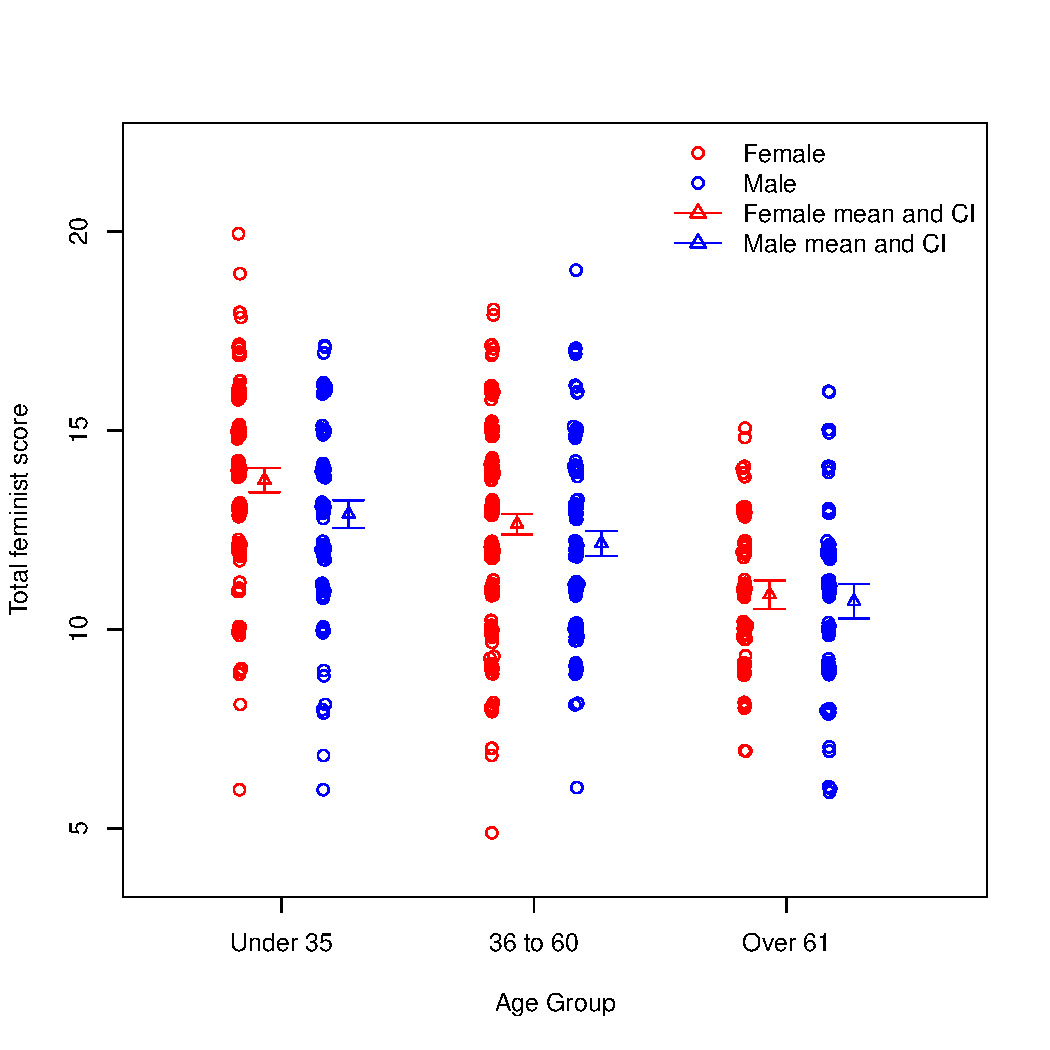
\includegraphics[height = 0.7\textwidth, keepaspectratio]{Figure/oth1}
  %\vspace{-20pt}
  %\caption{Boxplots of PM10 in 2006--2012}
  \label{fig:oth1}
\end{figure}
\end{frame} 


\begin{frame}[fragile]
  \frametitle{Lattice plots}

\begin{figure}[h]
  \vspace{-20pt}
  \centering
  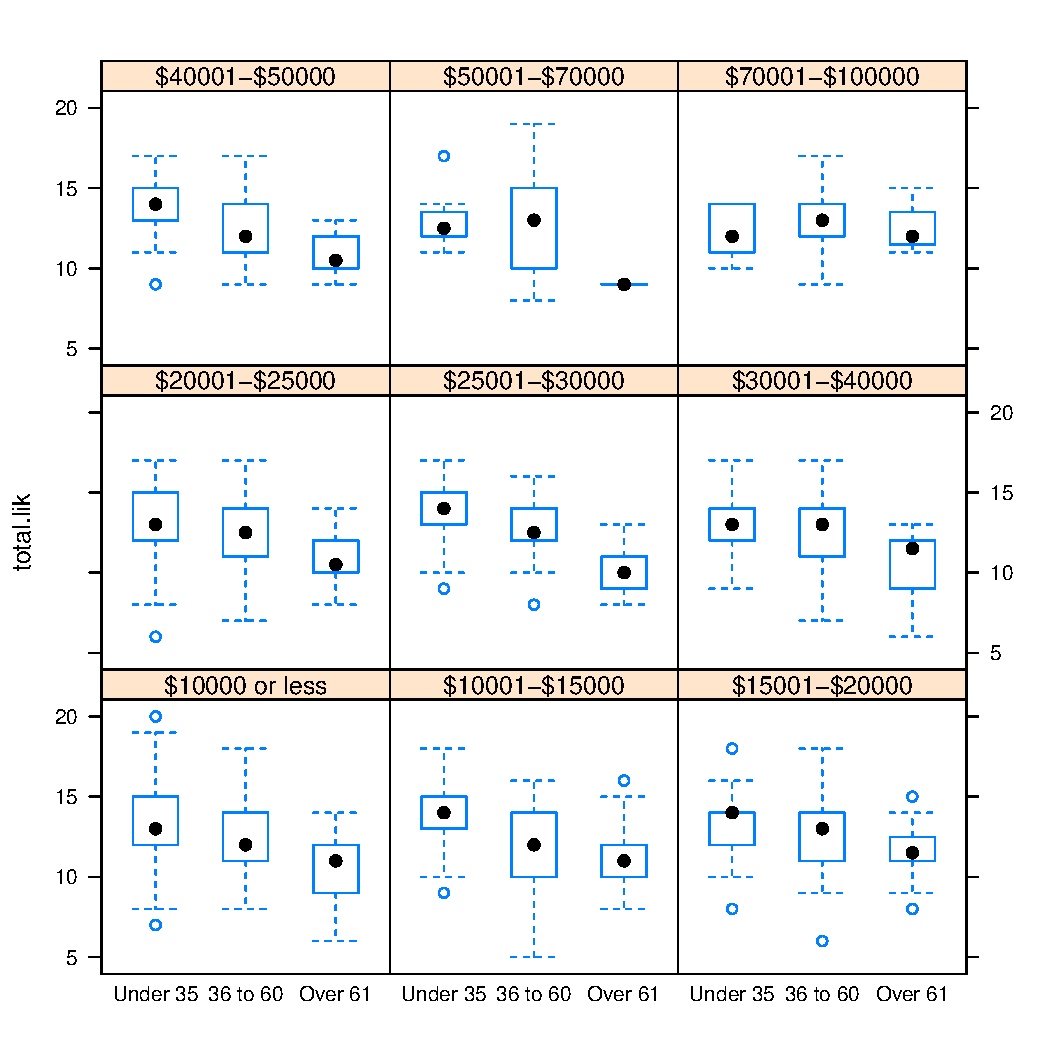
\includegraphics[height = 0.7\textwidth, keepaspectratio]{Figure/oth2}
  %\vspace{-20pt}
  %\caption{Boxplots of PM10 in 2006--2012}
  \label{fig:oth2}
\end{figure}
\end{frame} 
\end{document}     
